\section{Real time-series illustrations: series, trends and selectors}
\label{sec:expanded-applications}
The final illustration is deliberately separate
from the computational timings. It tests how
the selected \emph{level} of smoothing and
the polynomial order affect an interpretable
trend rather than claiming to produce a
new stochastic forecast.

\subsection{Datasets and common candidate protocol}
We use two frozen monthly public series:
the Mauna Loa atmospheric CO$_2$ mean
($n=441$, January 1990--September 2026,
parts per million) and the monthly
US effective federal funds rate
($n=201$, January 2010--September 2026,
percent, not seasonally adjusted)
\cite{noaa2026mlo,fred2026fedfunds}.
The first contains a strong seasonal
component around long-run growth;
the second contains abrupt shifts
and extended low-rate periods.
Both are useful for illustrating how
different time scales affect
trend estimation.

For each series, the archived study
uses $d\in\{1,2,3,4\}$,
$\mu=0$ or a training-derived
$\operatorname{mean}(D_d y_{\rm train})$,
and CV, GCV, AICc, BIC,
conditional Gaussian profile MLE,
and controlled $S=0.86$.
The first five optimize their
preexisting scores over the \emph{same}
29-point finite $S$ candidate grid;
the controlled option selects $S$
by prescription rather than
minimization. Consequently a
selected $S=0.1$ or $S=0.98$
may merely be a \emph{grid
boundary} optimum.

\subsection{Observed series and four selected trends}
Figure~\ref{fig:expanded-actual-trends}
plots the \emph{observed monthly values}
and fitted trends at the
stored $d=2$, fixed $\mu=0$
parameters for four contrasting
procedures. This view makes
visible the substantive consequences
of the selection table rather
than relying on numerical RMSE
alone. Curves are recomputed
deterministically at the
saved $(\lambda,\mu)$; no
statistical criterion is
optimized to create the figure.

\begin{figure}[tbp]
\centering
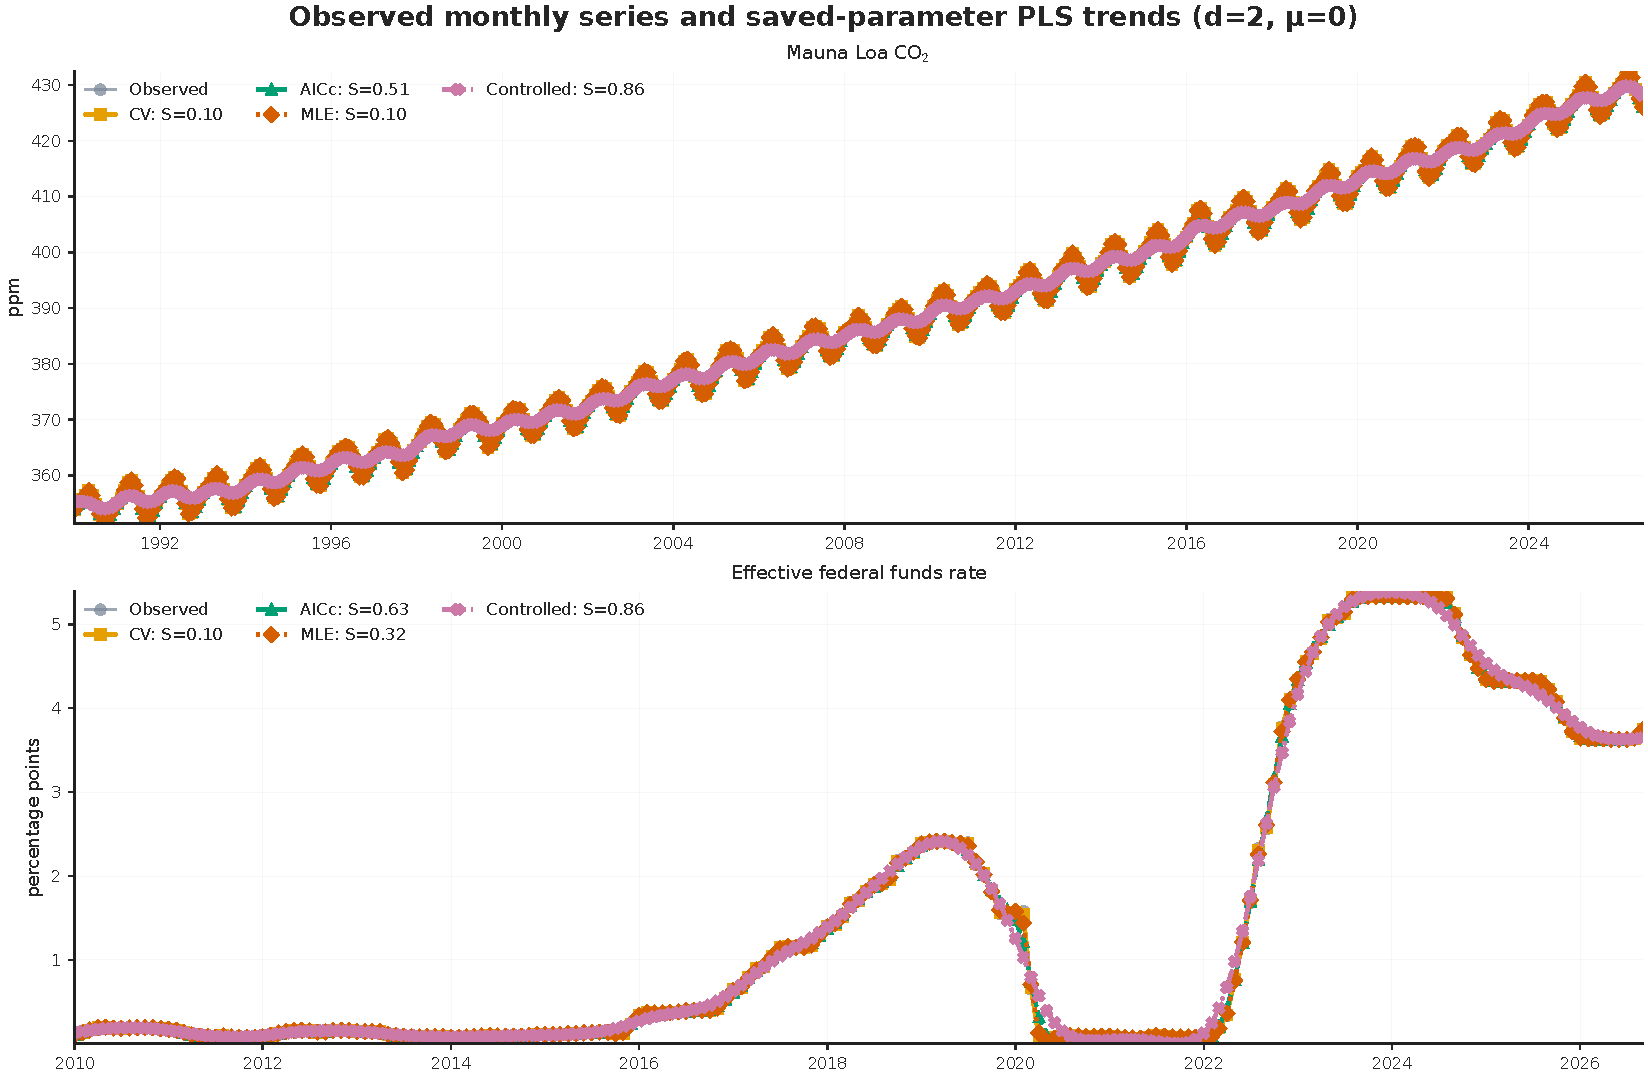
\includegraphics[width=\linewidth]{figures/sncs_observed_trends.pdf}
\caption{Frozen monthly observations
(gray) and in-sample penalized
least-squares trends for CV,
AICc, conditional MLE and
prescribed $S=0.86$,
with $d=2$ and fixed $\mu=0$.
The chosen penalty and resulting
smoothness level are drawn
from saved experiment JSON.
Coincident curves may overlap.
These are two-sided
historical smoothers, not
future forecasts.}
\label{fig:expanded-actual-trends}
\end{figure}

\begin{table}[tbp]
\centering\footnotesize
\caption{Empirical $d=2$, $\mu=0$
comparison for the two full
series. $\lambda$ and $S$
are selected in-sample;
RMSE and MAE compare a
separately extrapolated
historical 12-month holdout
against raw observations.
The 29-point search grid
is finite, and the
single-origin holdout
does not establish
predictive superiority.}
\label{tab:expanded-realdata}
\begin{tabular}{llrrrr}
\toprule
Series & Criterion & $\lambda$ & $S$ & RMSE & MAE \\
\midrule
CO$_2$ & CV & 0.0205 & 0.100 & 3.328 & 2.839 \\
CO$_2$ & GCV & 0.0205 & 0.100 & 3.328 & 2.839 \\
CO$_2$ & AICc & 0.428 & 0.509 & 3.413 & 2.930 \\
CO$_2$ & BIC & 0.0205 & 0.100 & 3.328 & 2.839 \\
CO$_2$ & MLE & 0.0205 & 0.100 & 3.328 & 2.839 \\
CO$_2$ & Controlled & 41.8 & 0.860 & 2.162 & 1.820 \\
\midrule
FEDFUNDS & CV & 0.0205 & 0.100 & 0.512 & 0.495 \\
FEDFUNDS & GCV & 0.0205 & 0.100 & 0.512 & 0.495 \\
FEDFUNDS & AICc & 1.21 & 0.634 & 0.538 & 0.522 \\
FEDFUNDS & BIC & 0.0205 & 0.100 & 0.512 & 0.495 \\
FEDFUNDS & MLE & 0.12 & 0.320 & 0.519 & 0.503 \\
FEDFUNDS & Controlled & 39.6 & 0.860 & 0.549 & 0.531 \\
\bottomrule
\end{tabular}

\end{table}

\subsection{Why the difference order matters even at equal $S$}
A simple but important geometric
point is that the same normalized
trace smoothness does not imply
the same fitted curve. At $d=1$,
the limiting zero-reference
trend is constant. At $d=2$,
it is linear; larger orders
allow correspondingly
higher-degree polynomial
null spaces. As a result,
the finite-$\lambda$ curves
with the same normalized
$S=0.86$ differ as well.
Figure~\ref{fig:expanded-orders}
plots all four orders for both
series, using the same prescribed
smoothness instead of pretending
that equal $\lambda$ values
have a comparable meaning.

\begin{figure}[tbp]
\centering
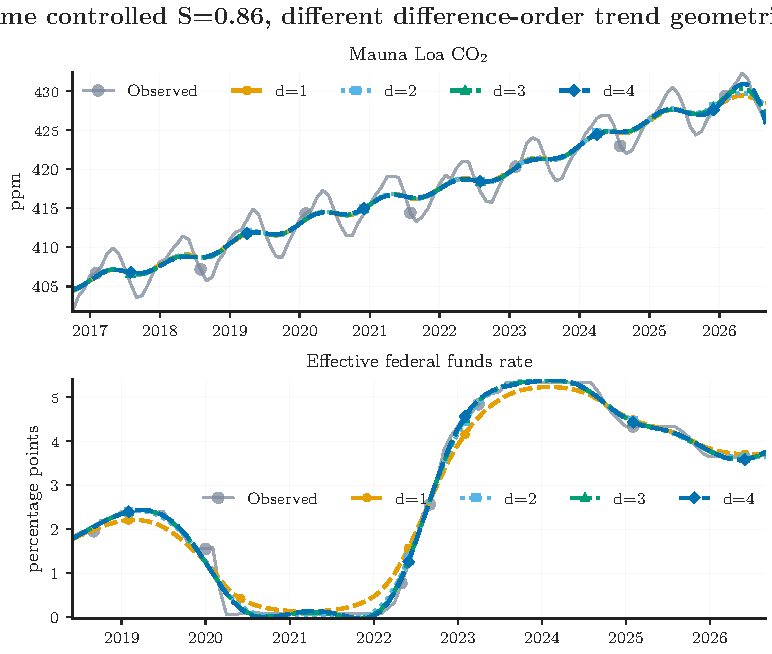
\includegraphics[width=\linewidth]{figures/sncs_orders_trends.pdf}
\caption{The most recent monthly
observations and four estimated
trends at the \emph{same}
controlled normalized
$S=0.86$ under
$d=1,2,3,4$, fixed $\mu=0$.
The variation across panels
is due to the finite-difference
order and its different
null-space geometry, not to
a change in the prescribed
fraction of trace smoothness.}
\label{fig:expanded-orders}
\end{figure}

\subsection{Criteria and data-derived reference differences}
Figure~\ref{fig:expanded-dashboard} uses
the archived selection and holdout
matrices to show two different
questions on a common $4\times6$
layout: how much smoothness is
selected, and how much
one-origin error is incurred
by the \emph{separate}
extrapolation rule.
The corresponding data-derived
$\mu$ figure, full 24-panel
trend/forecast collections,
and the most recent 120-month
CO$_2$ subset are provided
as supplementary figures.
For $\mu$ estimated from
observed differences, the
numeric value is computed
\emph{before} choosing the
penalty and separately for
each historical training window.

\begin{figure}[tbp]
\centering
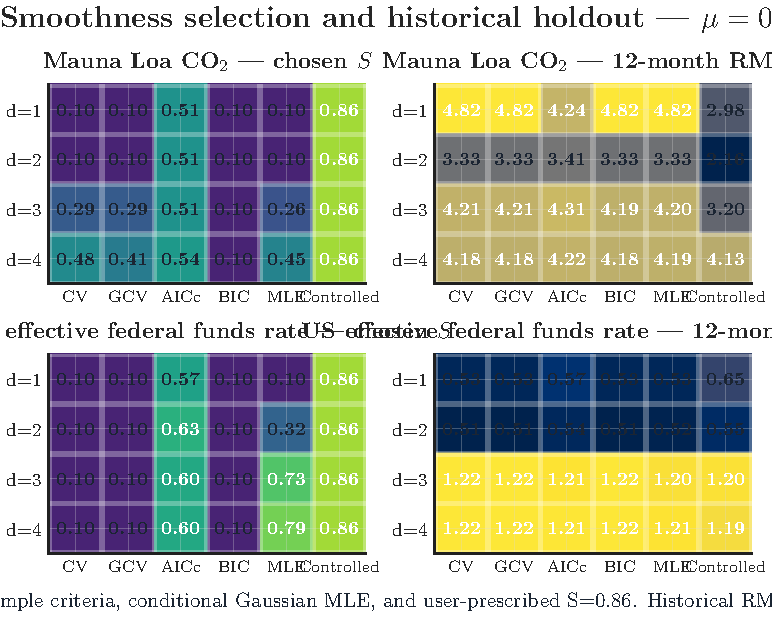
\includegraphics[width=\linewidth]{figures/sncs_compact_dashboard.pdf}
\caption{Saved smoothness
selection and historical
12-month holdout errors for
the two observed series,
four difference orders,
and six policies under
$\mu=0$. The six columns
include one prescribed
smoothness level and five
distinct in-sample
criterion objectives.
Only one historical
forecasting origin is
represented.}
\label{fig:expanded-dashboard}
\end{figure}

The extrapolation in the archive
is an explicit anchored local
polynomial fitted to the end
of each historical PLS trend,
not the PLS estimator itself.
For the historical holdout,
all mean and penalty
selections use the
training period only,
and the prediction error
is measured against
\emph{noisy observed values},
not the inaccessible
latent trend. For CO$_2$
the extrapolation has no
seasonal model; for the
federal funds rate it
does not model regime or
policy changes. Consequently
its one-origin errors
are illustrative diagnostics
and not the basis for
claiming that a particular
smoother or root algorithm
is a superior forecasting
method.
